\documentclass[11pt]{article}

\usepackage[T1]{fontenc}
\usepackage[utf8]{inputenc}
\usepackage[a4paper,margin=2.4cm]{geometry}
\usepackage{amsmath,amssymb,mathtools}
\usepackage{booktabs}
\usepackage{array}
\usepackage{xcolor}
\usepackage{enumitem}
\usepackage[expansion=false]{microtype}
\usepackage{pgfplots}
\pgfplotsset{compat=1.18}
\usepackage[hidelinks]{hyperref}
\setlength{\emergencystretch}{3em}

% ---- limiting-case tags ----
\definecolor{cNcol}{HTML}{1b6e1b}
\definecolor{cWcol}{HTML}{8a5a00}
\definecolor{cPcol}{HTML}{b00020}
\newcommand{\cN}{\textsuperscript{\textcolor{cNcol}{[N]}}}
\newcommand{\cW}{\textsuperscript{\textcolor{cWcol}{[W]}}}
\newcommand{\cP}{\textsuperscript{\textcolor{cPcol}{[P]}}}

% ---- symbol macros (mode-agnostic) ----
\newcommand{\fxy}{\ensuremath{f_{\mathrm{xy}}}}
\newcommand{\Kcw}{\ensuremath{K_{\mathrm{cw}}}}
\newcommand{\Bk}{\ensuremath{B_{k}}}
\newcommand{\Em}{\ensuremath{E_{\mathrm{m}}}}
\newcommand{\fd}{\ensuremath{f_{\mathrm{d}}}}
\newcommand{\fnn}{\ensuremath{f_{\mathrm{n}}}}
\newcommand{\Kow}{\ensuremath{K_{\mathrm{OW}}}}
\newcommand{\TSCF}{\ensuremath{\mathrm{TSCF}}}
\newcommand{\RCF}{\ensuremath{\mathrm{RCF}}}
\newcommand{\Lkg}{\ensuremath{\,\mathrm{L\,kg^{-1}}}}
\newcommand{\ffree}{\ensuremath{\varphi_{\mathrm{free}}}}

\newcommand{\boxnote}[1]{%
  \par\medskip\noindent\fcolorbox{black!55}{black!4}{%
  \begin{minipage}{0.985\linewidth}\small #1\end{minipage}}\par\medskip}

\title{\vspace{-1.2cm}\Large Theoretical anchor for the PFAS--rice $\fxy(n)$ functional form
and the IOC pH term\\[2pt]
\normalsize A standalone theory note for a four--compartment dynamic uptake model of
permanently--anionic PFAS in paddy rice (\textit{Oryza sativa})}
\author{}
\date{}

\begin{document}
\maketitle
\vspace{-1.4cm}

\noindent\textbf{Status.} Standalone note, executable independently of the S0--S5 handoff chain;
appendable to the model documentation. The empirical results of \S\ref{sec:emp} are taken as
\emph{given} (closed elsewhere); this note supplies only their \emph{theoretical} justification.
Limiting--case tags: \cN\,neutral non--electrolyte, \cW\,weak electrolyte (weak acid/base),
\cP\,permanent monovalent anion (PFAS, $\fd\!\approx\!1$, $z=-1$).

% =====================================================================
\section*{Verdict at a glance}
\addcontentsline{toc}{section}{Verdict at a glance}
\boxnote{%
\textbf{Task A.} \emph{Yes} --- the theory predicts a \textbf{monotonic decline} of $\fxy$ with
perfluorocarbon chain length $n$, not a Briggs bell. The bell is a property of the
\emph{neutral}--molecule trans-membrane permeability optimum; for a permanent anion its
\emph{rising} (left) limb is removed by three independent facts
[(i) $\fd\!\approx\!1\Rightarrow$ no ion trap; (ii) inside--negative $\Em\Rightarrow$ electrostatic
anion exclusion at all $n$; (iii) rising chain length $\Rightarrow$ rising root sorption $\Bk(n)\Rightarrow$
sequestration], leaving only the sorption--driven \emph{declining} limb. The natural bounded
closed form is the \textbf{logistic} $\fxy(n)=\eta/\!\left(1+\kappa\,10^{s n}\right)$; the
\emph{exponential tail} is simply its large--$n$ asymptote, so logistic and exponential are not
competitors. The predicted log-it slope $\beta=s\ln 10\approx 0.6$--$1.1\,\mathrm{C^{-1}}$ brackets
the empirical envelope $0.41$--$1.14$ (pooled $0.67$; OLS fit to \S\ref{sec:emp}a gives
$\beta=0.86$, $R^2=0.97$); the polar--end ceiling $\fxy(\mathrm{PFBA})=0.79\approx$ the Briggs
maximum $0.784$. This \emph{vindicates decision F1}: the bell/U-shaped \RCF{} belongs to root
\emph{sorption}, a separate compartment quantity, not to $\fxy$.\\[4pt]
\textbf{Task B.} \emph{Confirmed} --- in flooded paddy the pH effect on anion uptake enters
\textbf{mainly through $\Em$} (electrostatic / Nernst--Planck channel), \emph{not} through
speciation: with $\mathrm{pKa}\!\le\!1$ the neutral fraction is
$\fnn\!\approx\!10^{-5}$--$10^{-7}$ across pH $5.5$--$7.0$ and is pH--invariant in absolute terms,
so the weak--acid ion--trap lever is switched off. $\mathrm{NH_4^+}$ depolarisation
($-120\!\to\!-90$~mV) relaxes the exclusion factor $e^{N}$ from $107$ to $33$ ($\sim\!3.2\times$),
raising the passive anion influx $\sim\!2.5\times$. The pH--responsive congener \textbf{PFDA} is
explained by $\Em$ modulation (and possibly pH--dependent cell--wall charge in $\Kcw$) in the
steep low-$\fxy$ regime, \emph{not} by its own protonation. \textbf{Key data gap:} the in-situ
paddy $\Em$ ($-90$ to $-120$~mV $\Rightarrow$ $\sim\!2.5$--$3\times$ spread in passive influx).}

% =====================================================================
\section{Conventions and symbol map}\label{sec:conv}

Concentrations are mass per volume of water unless noted. $n$ is the total perfluorocarbon chain
length (PFBA $C_4\,\ldots\,$PFOA $C_8\,\ldots\,$PFTeDA $C_{14}$; sulfonates PFBS $C_4$,
PFHxS $C_6$, PFOS $C_8$). Head group: CA $=$ carboxylate, SA $=$ sulfonate. Paddy porewater pH
$5.5$--$7.0$; PFCA $\mathrm{pKa}\approx0$--$1$, PFSA $\mathrm{pKa}<0$, hence $\fd\approx1$, $z=-1$.
The tissue binding factor is
\begin{equation}\label{eq:Bk}
\Bk \;=\; \theta_k \;+\; f_{\mathrm{prot}}K_{\mathrm{prot}} \;+\; f_{\mathrm{PL}}K_{\mathrm{PL}}
\;+\; f_{\mathrm{cw}}\Kcw \qquad [\Lkg\ \text{dw}],
\end{equation}
with $\theta_k$ the tissue water $[\Lkg]$, $f_x$ component mass fractions $[\mathrm{kg\,kg^{-1}}]$,
$K_x$ partition coefficients $[\mathrm{L\,kg\text{-}component^{-1}}]$.

\begin{table}[h]
\centering\small
\renewcommand{\arraystretch}{1.15}
\caption{Symbol $\leftrightarrow$ source--symbol map and the limiting case each term belongs to.}
\label{tab:sym}
\begin{tabular}{@{}l >{\raggedright\arraybackslash}p{0.40\linewidth} >{\raggedright\arraybackslash}p{0.27\linewidth} c@{}}
\toprule
Note symbol & Source symbol (reference) & Meaning & Case\\
\midrule
$\fxy\in(0,1]$ & --- (new); TSCF analog, cf.\ Trapp \TSCF{} & root$\to$xylem loading factor & \cP\\
$\Kcw$ & $K_{cw}$, cuticle/wall--water (Trapp 2004, eq.~7) & cell-wall--water partition & \cN\cW\cP\\
$\Bk$ & composite of $K_{RW}$ terms (Trapp 2000, eq.~5) & tissue binding factor & all\\
$\RCF$ & $\RCF=K_{RW}$ (Briggs 1982; Trapp 2000) & root concentration factor & all\\
$\TSCF$ & \TSCF{} (Briggs 1982, eq.~3) & transpiration stream conc.\ factor & \cN\,(bell)\\
$\Em$ & $E$, $E_C=-0.12$~V (Trapp 2000, eqs.~6,8; Tab.~1) & plasmalemma potential & \cW\cP\\
$N$ & $N=zEF/RT$ (Trapp 2000, eq.~9) & electrochemical number & \cW\cP\\
$\fd,\ \fnn$ & $f_{df},\ f_{nf}$ (Trapp 2000, eqs.~12--13) & dissociated/neutral free fractions & \cW; \cP\,($\fd\!\approx\!1$)\\
$P_n,\ P_d$ & $P_n,\ P_d$ (Trapp 2000) & neutral/ion permeability & \cN\cW; \cP\\
$J_{\max},K_M$ & --- (new); Michaelis--Menten carrier & saturable carrier kinetics & \cP\\
$\Kow$ & $\Kow$ (Briggs 1982; Trapp) & octanol--water partition & \cN\cW\\
$\eta$ & --- (new) & xylem--loading transfer efficiency & \cP\\
$\ffree$ & mobile free fraction $=\theta/\Bk$ & free aqueous fraction in root & all\\
$s,\ \beta$ & $b=0.77$ (Briggs 1982, eq.~1) $\to$ slope & sorption / log-it slope per carbon & \cP\\
\bottomrule
\end{tabular}
\end{table}

% =====================================================================
\section{The governing cell model (Trapp ionizable--compound framework)}\label{sec:gov}

The four--compartment DPU of Rein et al.\ (2011) and Brunetti et al.\ (2019) is, at the
membrane level, the Trapp (2000, 2004) ionizable--compound cell model. Its primitive fluxes are:

\noindent\textbf{Neutral flux \cN\cW}\ (Fick; Trapp 2000 eq.~1, 2004 eq.~1):
\begin{equation}\label{eq:fick}
J_n \;=\; P_n\,(a_{n,o}-a_{n,i}).
\end{equation}

\noindent\textbf{Ion flux \cW\cP}\ (Nernst--Planck / Goldman--Hodgkin--Katz; Trapp 2000 eqs.~8--9):
\begin{equation}\label{eq:ghk}
\frac{a_i}{a_o}=e^{-N},\qquad
J_d \;=\; P_d\,\frac{N}{e^{N}-1}\,\bigl(a_{d,o}-a_{d,i}\,e^{N}\bigr),\qquad
N \equiv \frac{z\,\Em\,F}{RT}.
\end{equation}
For a monovalent anion ($z=-1$) and inside--negative $\Em=-0.12$~V at $T=298$~K
($F/RT=38.9~\mathrm{V^{-1}}$), $N=+4.67$ and $e^{N}\approx107$: the influx term is divided by
$e^{N}-1\approx106$, i.e.\ \emph{passive anion permeation is suppressed $\sim\!100\times$}
(electrostatic / Donnan exclusion). The Michaelis--Menten carrier overcomes this exclusion.

\noindent\textbf{Speciation \cW\cP}\ (Henderson--Hasselbalch; Trapp 2000 eqs.~10--11):
\begin{equation}\label{eq:hh}
\fnn=\frac{1}{1+10^{\,i(\mathrm{pH}-\mathrm{pKa})}}\quad(i=+1\ \text{acids}),
\qquad \fd=1-\fnn .
\end{equation}

\noindent\textbf{Sorption / RCF \cN\cW\cP}\ (Trapp 2000 eq.~5; our eq.~\ref{eq:Bk}):
$\RCF=K_{RW}=\theta+\sum_x f_xK_x$, reducing for neutrals to $W+Lc\Kow^{b}$.

\noindent\textbf{Xylem loading \cN}\ (detailed root model; Trapp 2000 eqs.~29--32). The shoot is
loaded by an apoplastic bypass fraction $\varepsilon$ ($\approx5\%$) of the transpiration stream
\emph{plus} symplastic transfer, while a sorptive sink in the central cylinder
($K_{nZ}\propto\Kow$, eq.~32) depletes the ascending xylem; the model TSCF is
$f_{fZ}\,C_Z/C_S$ with $f_{fZ}=1/(K_{RX}+K_{nZ})$.

\noindent\textbf{Briggs neutral relationships \cN}\ (Briggs 1982 eqs.~1--3; Trapp 2004 eqs.~4--6b):
\begin{align}
\TSCF &= 0.784\,\exp\!\Bigl[-\tfrac{(\log\Kow-1.78)^2}{2.44}\Bigr], \label{eq:briggsT}\\
\RCF &= 0.82 + 10^{\,0.77\log\Kow-1.52}, \qquad
\log\RCF_{\text{macerated}} = 0.77\log\Kow-1.52. \label{eq:briggsR}
\end{align}
Equation~\eqref{eq:briggsT} is the \emph{bell} (peak at $\log\Kow\approx1.8$, maximum $0.784$),
fitted to 17 \emph{non--ionised} compounds. Equation~\eqref{eq:briggsR} shows the RCF as a constant
water/free--space floor ($0.82$) plus a lipophilic--sorption term with slope $b=0.77$.

\boxnote{\textbf{Why these are the right primitives.} The bell \eqref{eq:briggsT} arises from a
\emph{competition} internal to the neutral molecule: on the polar side, low membrane permeability
$P_M=10^{\,1.2\log\Kow-7.5}$ (Trapp 2004 eq.~2c) limits entry; on the lipophilic side, sorption to
the central cylinder \eqref{eq:briggsR}-type term depletes the xylem. Both limbs are tied to
\emph{neutral} lipophilicity. The questions for PFAS are therefore: which of these limbs survive
when the molecule is a permanent anion, and what replaces $\log\Kow$ as the chain-length axis.}

% =====================================================================
\section{Task A --- why $\fxy(n)$ is a monotonic decline}\label{sec:A}

\subsection{Hybrid root influx and the definition of $\fxy$}
For a permanent anion the membrane influx is the sum of a strongly suppressed passive term and a
carrier term (the neutral term being negligible, eq.~\ref{eq:hh}):
\begin{equation}\label{eq:jR}
j_R \;=\;
\underbrace{P_d\,\frac{N}{e^{N}-1}\,\fd\,C_o}_{\text{GHK anion ($\times\,e^{-N}$ excluded)}}
\;+\;\underbrace{P_n\,\fnn\,C_o}_{\approx\,0}
\;+\;\underbrace{\frac{J_{\max}C_o}{K_M+C_o}}_{\text{carrier}} .
\end{equation}
We factor the loading factor into a (chain--length--independent) electrochemical transfer
efficiency and a (chain--length--dependent) mobile free fraction in the root,
\begin{equation}\label{eq:factor}
\boxed{\;\fxy(n) \;=\; \eta(\Em,\ \text{carrier})\;\times\;\ffree(n)\;}
\qquad \eta\le 1,
\end{equation}
where $\eta$ collects the apoplastic bypass $\varepsilon$ and the carrier-mediated symplastic
transfer net of back-diffusion (set by charge / $\Em$, hence essentially independent of tail
length), and $\ffree$ is the fraction of root-internal PFAS that remains in the mobile aqueous
phase available for xylem loading.

\subsection{The mobile free fraction $\Rightarrow$ a logistic in $n$}
Of the total PFAS held in the root tissue, the mobile aqueous fraction is
\begin{equation}\label{eq:phifree}
\ffree(n)=\frac{\theta_R}{\Bk(n)},\qquad
\Bk(n)=\theta_R+f_{\mathrm{cw}}\Kcw(n)+f_{\mathrm{PL}}K_{\mathrm{PL}}(n)+f_{\mathrm{prot}}K_{\mathrm{prot}}(n).
\end{equation}
By the Collander linear--free--energy relationship (the basis of Briggs eq.~\ref{eq:briggsR}), each
added perfluorocarbon contributes a roughly constant increment to the free energy of sorption, so
every partition coefficient grows \emph{log--linearly} with $n$, $K_x(n)=K_x^{0}\,10^{s_x n}$. When
one sorptive term dominates (membrane/protein binding at long chains),
$\Bk(n)\approx\theta_R\bigl(1+\kappa\,10^{s n}\bigr)$ with $\kappa=f_xK_x^{0}/\theta_R$, whence
\begin{equation}\label{eq:logistic}
\boxed{\;\ffree(n)=\frac{1}{1+\kappa\,10^{s n}}=\frac{1}{1+10^{\,s(n-n_0)}}\;},
\qquad n_0=-\frac{\log\kappa}{s}.
\end{equation}
This is exactly a \textbf{logistic} (sigmoid) in $n$. Combining with eq.~\eqref{eq:factor},
$\fxy(n)=\eta/\!\left(1+10^{\,s(n-n_0)}\right)$, and in the small-$\fxy$ regime ($n\gtrsim5$)
\begin{equation}\label{eq:logit}
\operatorname{logit}\fxy \equiv \ln\frac{\fxy}{1-\fxy}\;\approx\;\alpha-\beta\,n,
\qquad \beta=s\ln 10,\qquad \alpha=\ln\eta+\beta\,n_0 .
\end{equation}
The adopted two--parameter form $\operatorname{logit}\fxy=\alpha-\beta n$ is therefore the
\emph{large-$n$ linearisation} of the bounded logistic \eqref{eq:logistic}, and the bound itself
is the physically required ceiling $\fxy\le\eta\le1$.

\subsection{Logistic vs.\ exponential tail --- not competitors}
The logistic \eqref{eq:logistic} contains both regimes:
\[
\begin{aligned}
\text{short chain }(\kappa\,10^{sn}\!\ll\!1):&\quad \fxy\to\eta\ \ (\le1;\ \text{the DPU base }\fxy{=}1\text{ when }\eta{=}1),\\[2pt]
\text{long chain }(\kappa\,10^{sn}\!\gg\!1):&\quad \fxy\to\frac{\eta}{\kappa}\,10^{-sn}\ \ \text{(exponential tail)},
\end{aligned}
\]
i.e.\ the \textbf{exponential tail is the large-$n$ asymptote of the logistic}. The logistic is the
preferred closed form because it (a) is bounded in $(0,1]$ by construction --- a fraction cannot
exceed unity, and the unrestricted DPU base $\fxy=1$ (assumption A2) is its $n\to-\infty$ limit;
(b) needs only two parameters; (c) reproduces the observed short--chain plateau \emph{and} the
exponential long--chain decay with a single function. A bare exponential $\fxy=e^{\alpha-\beta n}$
would exceed $1$ for small $n$ and cannot encode the DPU ceiling.

\subsection{Why there is no bell --- removal of the rising limb}
The Briggs bell \eqref{eq:briggsT} owes its \emph{rising} limb to neutral-molecule permeability
turning on with lipophilicity. For a permanent anion this limb is removed by three independent
facts, exactly as posited:
\begin{enumerate}[leftmargin=1.4em,itemsep=2pt]
\item \textbf{$\fd\approx1\Rightarrow$ no ion trap.} The ion trap --- the \emph{dominant}
accumulation mechanism for monovalent weak electrolytes (Trapp 2000) --- requires a neutral form
that diffuses quickly and dissociates in an alkaline compartment. With $\fnn\approx0$
(eq.~\ref{eq:hh}) there is no neutral form to trap, so the pH-driven peak that lifts weak-acid
uptake never forms.\cP
\item \textbf{Inside--negative $\Em\Rightarrow$ electrostatic exclusion at all $n$.} The GHK influx
\eqref{eq:ghk} is suppressed by $e^{N}\approx107$ independently of chain length, so the anion does
not ``turn on'' as lipophilicity rises; passive entry is capped low for every congener.\cP
\item \textbf{Rising chain length $\Rightarrow$ rising sorption $\Rightarrow$ sequestration.} $\Bk$
rises $\sim\!3$ orders from $C_4$ to $C_{12}$ (root $\Bk$: PFBA $\approx1.7$, PFOA $\approx23$,
PFDoDA $\approx1075\Lkg$~dw). Through eq.~\eqref{eq:phifree} this monotonically lowers $\ffree$ and
hence $\fxy$.\cP
\end{enumerate}
With the rising limb gone, only the sorption--driven \emph{declining} limb survives; the result is
a \textbf{monotonic decline}.

\subsection{Slope, ceiling, and head group from first principles}
\textbf{Slope.} From eq.~\eqref{eq:logit}, $\beta=s\ln10$ with $s=b_{\mathrm{sorp}}\times
(\Delta\log\Kow\ \text{per CF}_2)$. Using the Briggs sorption slope $b_{\mathrm{sorp}}=0.77$ and
$\Delta\log\Kow\approx0.5$--$0.6$ per CF$_2$ gives $\beta\approx0.9$--$1.1\,\mathrm{C^{-1}}$;
because PFAS membrane/protein sorption slopes are typically \emph{shallower} than octanol
($b_{\mathrm{sorp,eff}}\approx0.5$--$0.6$), the bracket extends down to
$\beta\approx0.6$--$0.7\,\mathrm{C^{-1}}$. Predicted bracket $\beta\in[0.6,1.1]\,\mathrm{C^{-1}}$.

\noindent\textbf{Ceiling.} $\eta$ caps the polar end. PFBA realises $\fxy=0.79$, essentially the
Briggs maximum $0.784$ \eqref{eq:briggsT}: the shortest, most water-like PFAS reaches the same
\emph{passive transpiration-sweep ceiling} that the neutral bell peaks at --- but approached from
the polar side, so only the $C_4$ member attains it, whereas neutrals reach it at intermediate
$\log\Kow\approx1.8$.

\noindent\textbf{Head group.} A sulfonate adds a near-constant binding increment; in the
linear--free--energy picture this is an additive offset to $\alpha$,
$\fxy^{\mathrm{SA}}\approx\fxy^{\mathrm{CA}}\,e^{-1.5}$, equivalent to
$\Delta\alpha=-1.5$ or $\approx+1.8$--$2.2$ ``effective carbons'' of extra sorption. Treated as a
sensitivity term (sign uncertain; one crop reversed it at $C_4$).

\subsection{Vindication of decision F1 (bell/U $\RCF$ $\to$ root sorption, not $\fxy$)}
$\RCF$ and $\fxy$ are \emph{different} quantities. By eq.~\eqref{eq:briggsR}/\eqref{eq:phifree},
$\RCF=$ apparent-free-space/water floor ($\approx0.2$ in Trapp's detailed root model; $0.82$ in the
Briggs water term) $+$ a sorption term $\propto\Bk(n)$ that rises monotonically. A
bell/U-shaped \RCF{} can arise from the sorption rise (optionally with low-$n$ carrier accumulation
on the polar side), and it is a \emph{root-compartment} property. $\fxy$ is the \emph{xylem-loading
efficiency}, governed by $\ffree$ and $\eta$. Trapp (2000) builds exactly this two-process
decomposition --- RCF dominated by sorption (eq.~5), TSCF limited by central-cylinder loading
(eqs.~29--32). Assigning the bell/U to \RCF{} (sorption) while keeping $\fxy$ monotonic is therefore
\emph{internally consistent with the source framework}, not an \emph{ad hoc} split. \textbf{F1 is
vindicated.}

\subsection{Consistency with the empirical results of \S\ref{sec:emp}}
Table~\ref{tab:check} and Fig.~\ref{fig:fxy} compare theory and the given empirics.

\begin{table}[h]
\centering\small
\renewcommand{\arraystretch}{1.2}
\caption{Theory vs.\ the given empirical results (\S\ref{sec:emp}).}
\label{tab:check}
\begin{tabular}{@{}l l l c@{}}
\toprule
Feature & Theory predicts & Empirical (given) & Match\\
\midrule
Shape vs.\ $n$ & monotonic decline (no bell) & monotonic decline & \checkmark\\
Closed form & bounded logistic (exp.\ tail = asymptote) & logistic, $\operatorname{logit}\fxy=\alpha-\beta n$ & \checkmark\\
Slope $\beta$ & $0.6$--$1.1\,\mathrm{C^{-1}}$ (LFER) & $0.41$--$1.14$ (pooled $0.67$; OLS $0.86$) & \checkmark\\
Polar ceiling & $\to$ Briggs max $0.784$ & $\fxy(\mathrm{PFBA})=0.79$ & \checkmark\\
Long-chain level & exp.\ tail $\ll0.1$ & $\fxy(\mathrm{PFTeDA})=5.2\times10^{-4}$ & \checkmark\\
Head group & SA $<$ CA (const.\ offset) & $\fxy^{\mathrm{SA}}\!\approx\!\fxy^{\mathrm{CA}}e^{-1.5}$ & \checkmark\\
Bell/U RCF & belongs to sorption, not $\fxy$ (F1) & assigned to root sorption & \checkmark\\
\bottomrule
\end{tabular}
\end{table}

\begin{figure}[h]
\centering
\begin{minipage}{0.49\linewidth}\centering
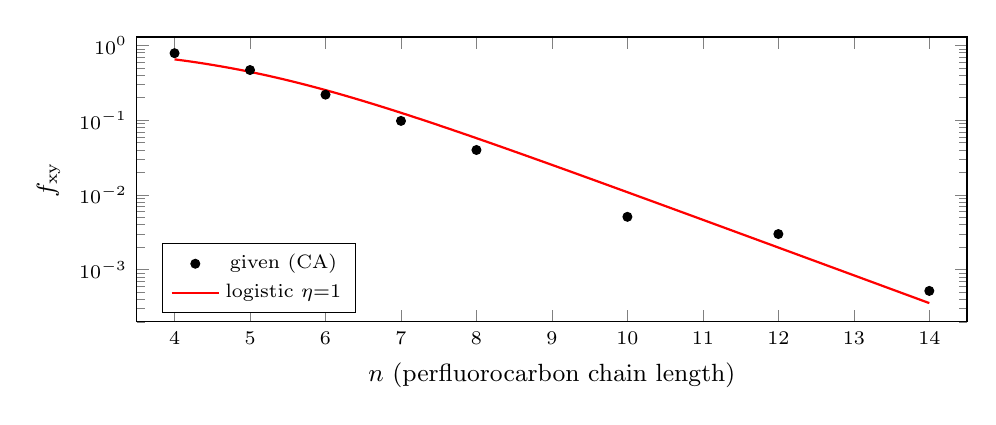
\begin{tikzpicture}
\begin{axis}[width=\linewidth,height=5.2cm,ymode=log,
  xlabel={$n$ (perfluorocarbon chain length)},ylabel={$\fxy$},
  xmin=3.5,xmax=14.5,ymin=2e-4,ymax=1.3,
  legend style={font=\scriptsize,at={(0.03,0.03)},anchor=south west},
  tick label style={font=\scriptsize},label style={font=\small}]
\addplot[only marks,mark=*,mark size=1.6pt] coordinates {
 (4,0.79)(5,0.47)(6,0.22)(7,0.098)(8,0.040)(10,0.0051)(12,0.0030)(14,0.00052)};
\addlegendentry{given (CA)}
\addplot[red,thick,domain=4:14,samples=120]{1/(1+exp(0.857*x-4.061))};
\addlegendentry{logistic $\eta{=}1$}
\end{axis}
\end{tikzpicture}\\[-1pt]{\scriptsize (a) monotonic decline on log axis}
\end{minipage}\hfill
\begin{minipage}{0.49\linewidth}\centering
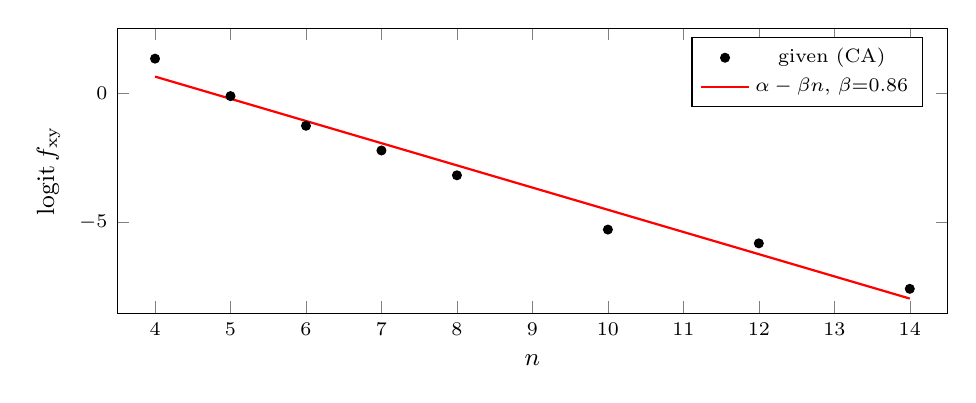
\begin{tikzpicture}
\begin{axis}[width=\linewidth,height=5.2cm,
  xlabel={$n$},ylabel={$\operatorname{logit}\fxy$},
  xmin=3.5,xmax=14.5,ymin=-8.5,ymax=2.5,
  legend style={font=\scriptsize,at={(0.97,0.97)},anchor=north east},
  tick label style={font=\scriptsize},label style={font=\small}]
\addplot[only marks,mark=*,mark size=1.6pt] coordinates {
 (4,1.325)(5,-0.120)(6,-1.266)(7,-2.220)(8,-3.178)(10,-5.274)(12,-5.806)(14,-7.561)};
\addlegendentry{given (CA)}
\addplot[red,thick,domain=4:14]{4.061-0.857*x};
\addlegendentry{$\alpha-\beta n$, $\beta{=}0.86$}
\end{axis}
\end{tikzpicture}\\[-1pt]{\scriptsize (b) log-it--linear ($R^2{=}0.97$)}
\end{minipage}
\caption{The given $\fxy(n)$ (central CA estimates, \S\ref{sec:emp}a) on (a) a log axis with the
logistic eq.~\eqref{eq:logistic} and (b) the log-it--linear form eq.~\eqref{eq:logit}. The
short--chain plateau (PFBA near the Briggs ceiling) and the exponential long--chain tail are the two
asymptotes of the same logistic.}
\label{fig:fxy}
\end{figure}

\subsection*{VERDICT (Task A)}
\boxnote{The Trapp ionizable--compound cell model plus the Briggs neutral relationships predict a
\textbf{monotonic} $\fxy(n)$ for permanent anions (the bell's rising limb is removed by
$\fd\!\approx\!1$, $\Em$ exclusion, and rising $\Bk$). The \textbf{logistic}
$\fxy=\eta/(1+\kappa\,10^{sn})$ is the natural bounded closed form, with the exponential tail as its
large-$n$ asymptote and the log-it--linear form as its small-$\fxy$ linearisation. Predicted slope
$\beta\in[0.6,1.1]\,\mathrm{C^{-1}}$ and ceiling $\to0.784$ reproduce the given envelope
($0.41$--$1.14$; PFBA $0.79$). The bell/U-shaped \RCF{} belongs to root \emph{sorption}, a separate
compartment quantity --- \textbf{decision F1 is vindicated.}}

% =====================================================================
\section{Task B --- the IOC pH term (F4)}\label{sec:B}

Three channels can in principle carry a pH/porewater dependence into anion uptake and $\fxy$:
\emph{speciation} (Henderson--Hasselbalch / ion trap), \emph{electrostatic} ($\Em$ via GHK),
and \emph{activity} (ionic strength via Davies). We evaluate each for the paddy case.

\paragraph{(1) Speciation channel --- frozen.\cP}
With $\mathrm{pKa}\le1$, eq.~\eqref{eq:hh} gives $\fnn\approx10^{-5}$--$10^{-7}$ across pH
$5.5$--$7.0$ (e.g.\ $\fnn=3\times10^{-6}$ at pH~5.5, $1\times10^{-7}$ at pH~7.0 for
$\mathrm{pKa}=0$). The neutral fraction is not merely small but \emph{pH--invariant in absolute
terms}; $\partial\fnn/\partial\mathrm{pH}$ is negligible. The ion-trap lever that governs weak-acid
pH dependence (Trapp 2000, \S4.7.5) is therefore switched off for PFAS.

\paragraph{(2) Electrostatic channel --- the live lever.\cP}
The exclusion factor is $e^{N}$ with $N=z\Em F/RT=-\Em F/RT$ (anion). $\Em$ is set kinetically by
the plasmalemma $\mathrm{H^+}$--ATPase and the permeant--ion gradients, so porewater chemistry acts
\emph{through} $\Em$:
\begin{equation}\label{eq:depol}
\begin{aligned}
\Em=-120~\mathrm{mV}:&\quad N=4.67,\ e^{N}=107,\ \tfrac{N}{e^{N}-1}=0.044;\\
\Em=-90~\mathrm{mV}\ (\mathrm{NH_4^+}\text{ depol.}):&\quad N=3.50,\ e^{N}=33,\
\tfrac{N}{e^{N}-1}=0.109.
\end{aligned}
\end{equation}
In flooded, anaerobic paddy soil $\mathrm{NH_4^+}$ is the dominant mineral-N species and
\emph{depolarises} the membrane ($-120\!\to\!-90$~mV), \emph{relaxing} the exclusion factor $e^{N}$
from $107$ to $33$ ($\sim\!3.2\times$) and raising the passive anion influx
$\sim\!2.5\times$ (the GHK factor $N/(e^N-1)$). This is the principal route by which pH and
porewater composition modulate PFAS loading.

\paragraph{(3) Activity channel --- secondary.\cP}
The Davies equation (Trapp 2000 eq.~7), $\log\gamma_d=-Az^2\!\left[\sqrt{I}/(1+\sqrt{I})-0.2I\right]$,
gives $\gamma_d\approx0.7$ for a monovalent ion at $I=0.5$~M. External/porewater ionic strength is
low and is neglected for the external and xylem phases in the source model; this channel is a
second-order correction.

\paragraph{PFDA --- the pH--sensitive congener.\cP}
PFDA ($C_{10}$ PFCA) is still a permanent anion ($\mathrm{pKa}\le1$), so its empirical pH
sensitivity \emph{cannot} come from its own protonation. The IOC framework attributes it to the
\emph{electrostatic} channel acting in the steep, low-$\fxy$ / high-sorption regime: PFDA sits where
$\fxy\approx5\times10^{-3}$, so a small $\Delta\Em$ (driven by porewater pH/$\mathrm{NH_4^+}$)
produces a large \emph{fractional} change in the already-tiny $\fxy$ and in $\RCF$, because the
influx scales with $e^{-N}$ (eq.~\ref{eq:depol}). A plausible amplifier is a pH--dependent
\emph{cell-wall Donnan charge}: pectic galacturonic carboxyls ($\mathrm{pKa}\approx3$--$4$)
deprotonate as pH rises, altering the wall's fixed charge and hence the electrostatic component of
$\Kcw$ for the anion. Both routes are accommodated by the IOC framework; \emph{neither} invokes
PFDA speciation.

\paragraph{Data gap.}
The in-situ paddy $\Em$ is unmeasured. The plausible range $-90$ to $-120$~mV maps (eq.~\ref{eq:depol})
to a $\sim\!2.5$--$3\times$ spread in passive anion influx --- the dominant quantitative
uncertainty in the pH term, and the priority measurement.

\subsection*{VERDICT (Task B)}
\boxnote{For paddy (fully anionic, $\fd\!\approx\!1$) the pH effect on root uptake and $\fxy$ enters
\textbf{mainly through $\Em$} (the Nernst--Planck/GHK electrostatic channel), \emph{not} through
speciation: $\fnn\approx10^{-5}$--$10^{-7}$ is negligible and pH-invariant, so the ion-trap lever is
off. The operative driver is $\mathrm{NH_4^+}$ depolarisation ($-120\!\to\!-90$~mV $\Rightarrow$
$e^{N}\,107\!\to\!33$, influx $\times2.5$), with activity ($\gamma_d$) and pH-dependent cell-wall
charge ($\Kcw$) as secondary corrections. \textbf{Scope note confirmed.} PFDA's pH response is the
$\Em$ (and possibly $\Kcw$) channel in the low-$\fxy$ regime, not its own protonation. The
unmeasured in-situ paddy $\Em$ is the key data gap.}

% =====================================================================
\section{Assumptions (explicit)}\label{sec:assume}
\begin{enumerate}[leftmargin=1.5em,itemsep=1pt,label=A\arabic*.]
\item PFAS are permanent monovalent anions over pH $5.5$--$7.0$: $\fd\approx1$, $\fnn\approx0$,
$z=-1$ (PFCA $\mathrm{pKa}\le1$, PFSA $<0$).
\item $\fxy$ factorises as $\eta(\Em,\text{carrier})\times\ffree(n)$ with $\eta$ chain-length
independent (charge-controlled), eq.~\eqref{eq:factor}.
\item All tissue partition coefficients $K_x(n)$ follow a Collander/Briggs log-linear (LFER)
dependence on $n$, with one sorptive term dominating at long chains, eqs.~\eqref{eq:phifree}--\eqref{eq:logistic}.
\item Root uptake is hybrid GHK + Michaelis--Menten (carrier overcomes anion exclusion),
eq.~\eqref{eq:jR}; passive neutral permeation is negligible.
\item $\Em$ is the sole significant route for porewater pH/ionic composition to modulate anion
loading (speciation frozen, activity secondary), \S\ref{sec:B}.
\item Constant-field (GHK) approximation, instantaneous cytoplasm--vacuole equilibrium, and the
two-process RCF/TSCF decomposition are inherited from Trapp (2000).
\item Empirical anchors ($\fxy$ table, $\beta$ envelope, ceiling, head-group offset, $\Bk$ values)
are taken as given (\S\ref{sec:emp}); this note justifies their form, not their values.
\end{enumerate}

% =====================================================================
\section{Empirical results justified (given; not re-derived)}\label{sec:emp}
\textbf{(a)} $\fxy(n)$ central (CA): $\{4{:}0.79,\,5{:}0.47,\,6{:}0.22,\,7{:}0.098,\,8{:}0.040,\,
10{:}5.1\!\times\!10^{-3},\,12{:}3.0\!\times\!10^{-3},\,14{:}5.2\!\times\!10^{-4}\}$;
logistic $\operatorname{logit}\fxy=\alpha-\beta n$, pooled $\beta\approx0.67\,\mathrm{C^{-1}}$
(per-crop/tissue $0.41$--$1.14$); level anchored on $\TSCF(\mathrm{PFBA})=0.79$, non-PFBA $C_4$--$C_{14}$
$\TSCF<0.3$; head group $\fxy^{\mathrm{SA}}\approx\fxy^{\mathrm{CA}}e^{-1.5}$.
\textbf{(b)} Root uptake carrier-mediated/partly active (Michaelis--Menten, inhibitor-sensitive);
bell/U-shaped RCF assigned to root sorption (decision F1).
\textbf{(c)} $\Bk$ rises $\sim\!3$ orders $C_4$--$C_{12}$ (root: PFBA $\approx1.7$, PFOA $\approx23$,
PFDoDA $\approx1075\Lkg$~dw).

% =====================================================================
\section*{References (with DOI status)}
\addcontentsline{toc}{section}{References}
\small
\begin{enumerate}[leftmargin=1.6em,itemsep=2pt]
\item Briggs G.G., Bromilow R.H., Evans A.A. (1982). Relationships between lipophilicity and root
uptake and translocation of non-ionised chemicals by barley. \textit{Pestic.\ Sci.}\ 13(5),
495--504. DOI: \texttt{10.1002/ps.2780130506}. \textcolor{cNcol}{[VERIFIED --- cross-referenced in
the Brunetti et al.\ 2019 reference list.]}
\item Trapp S. (2000). Modelling uptake into roots and subsequent translocation of neutral and
ionisable organic compounds. \textit{Pest Manag.\ Sci.}\ 56(9), 767--778. DOI:
\texttt{10.1002/1526-4998(200009)\-\allowbreak56:9<767::\-\allowbreak AID-PS198>\-\allowbreak3.0.CO;2-Q}. \textcolor{cNcol}{[VERIFIED ---
printed in the source PDF.]}
\item Trapp S. (2002). Dynamic root uptake model for neutral lipophilic organics. \textit{Environ.\
Toxicol.\ Chem.}\ 21(1), 203--206. DOI: not printed in the supplied PDF. \textcolor{cPcol}{[UNVERIFIED
--- bibliographic citation unambiguous; DOI not confirmable from the supplied materials, not
fabricated.]}
\item Trapp S. (2004). Plant uptake and transport models for neutral and ionic chemicals.
\textit{Environ.\ Sci.\ Pollut.\ Res.}\ 11(1), 33--39. DOI: \texttt{10.1065/espr2003.08.169}.
\textcolor{cNcol}{[VERIFIED --- printed in the source PDF.]}
\item Rein A., Legind C.N., Trapp S. (2011). New concepts for dynamic plant uptake models.
\textit{SAR QSAR Environ.\ Res.}\ 22(1--2), 191--215. DOI: \texttt{10.1080/1062936X.2010.548829}.
\textcolor{cNcol}{[VERIFIED --- printed in the source PDF.]}
\item Brunetti G., Kode\v{s}ov\'a R., \v{S}im\r{u}nek J. (2019). Modeling the translocation and
transformation of chemicals in the soil--plant continuum: a dynamic plant uptake module for the
HYDRUS model. \textit{Water Resour.\ Res.}\ 55(11), 8967--8989. DOI: \texttt{10.1029/2019WR025432}.
\textcolor{cNcol}{[VERIFIED --- printed in the source PDF.]}
\end{enumerate}

\end{document}
